% %%%%%%%%%%%%%%%%%%%%%%%%%%%%%%%%%%%%%%%%%%%%%%%%%%%%%%%%%%%%%%%%%%%%%%
% Dummy Chapter:
% %%%%%%%%%%%%%%%%%%%%%%%%%%%%%%%%%%%%%%%%%%%%%%%%%%%%%%%%%%%%%%%%%%%%%%

% %%%%%%%%%%%%%%%%%%%%%%%%%%%%%%%%%%%%%%%%%%%%%%%%%%%%%%%%%%%%%%%%%%%%%%
% The Introduction:
% %%%%%%%%%%%%%%%%%%%%%%%%%%%%%%%%%%%%%%%%%%%%%%%%%%%%%%%%%%%%%%%%%%%%%%
\fancychapter{Analysis}
\label{cap:Analysis}

\textit{Upon the experimental procedures, a developed pipeline was followed for the analysis of the RF, tuning and SM protocols, for each animal and imaging session. This process will be described hereby, along with the explanation of each utilized tool, analysis scripts and software. This chapter will first summarize the registration method utilized, the regions of interest selection technique, as well as the subsequent data treatment and used statistical tools. In particular, for this project's experiments' analysis, Suit2p software for automated selection of neurons in a raw image and corresponding fluorescence traces extraction was implemented. This package will here be concisely presented and compared with previously used methods.}

\section{Experiment's outputs}
\label{sec:Experimentsoutputs}

Once an experiment is completed, a set of raw images, as well as the corresponding stimuli information and event timings is available. For each protocol, there is a set of frames for every trial, according to the TPLSM system's scanning speed of $30 Hz$ ($6 Hz$ per plane). 
For instance, the RF protocol comprises 1120 trials and the triggers sent from bpod to the imaging computer for separating the movies come at each 4 trials. There are thus, for this case, 280 sets of images. Since each trial endures for $1s$, each of these sets contains 6 frames for each of the 4 relevant planes, prefacing, for the RF protocol, 24 total frames per trial. In turn, each of these frames contains a $512 \times 512$ pixels image of the fluorescent signals emitted from the animal's brain ($200 \mu m \times 200 \mu m$) and detected at that time (figure \ref{cm006}, for an example).
For each of the trial's sets of images, there is the corresponding stimulus information being saved in a Matlab structure: In the case of the RF, the changing feature is the position and the gratings direction order of the stimulus patch being presented in the screen during that trial, for the Tuning protocol these are the spacial and temporal frequencies as well as the direction of the centred stimulus, and finally for the SM protocol the independent variable is the stimulus type number. Apart from these, the constant features of the stimuli at each protocol are also saved in the same stimuli structure. 
The trial time stamps in bpod's triggering, states and Psychtoolbox's clocked timings from a received trigger to the next are also saved. This allows, in the latter analysis, to confirm and correct the stimuli information in the case of any eventual skipped trials.
Finally, Scan Image configurations are also saved, in each trial's video header, keeping the information required about the laser's power during that experiment, multiplane settings and read brightness offsets.

\begin{figure}[H] \centering 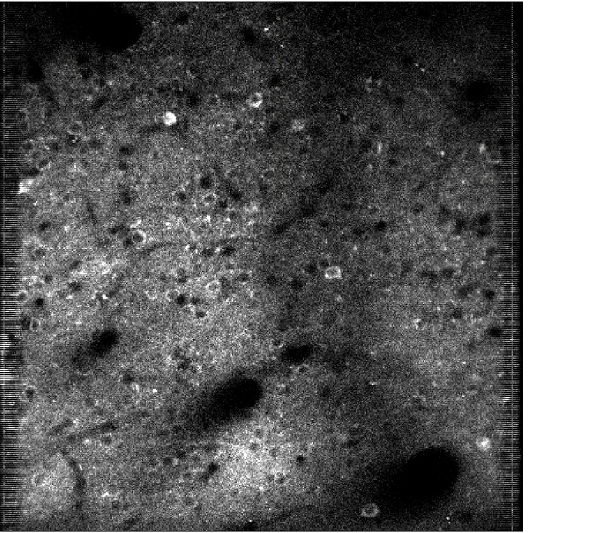
\includegraphics[width=10cm,height=10cm,keepaspectratio]{Figures/7.Results/ftraces/CM006.png} 
\caption{Average image of an example plane of imaging recordings across a session from an example animal. The full image corresponds to a $512\times 512$ map of $400 \mu m \times 400 \mu m$ of mouse V1 area, chosen as to respond to the center of the visual field of view.
\label{cm006}}
\end{figure}
\section{Images pre-processing: Separating planes and registration}
\label{sec:PreProcessing}

Each imaging raw movie intertwines the frames of each of the 4 planes. We used a software developed in the cortical circuits laboratory that parses and enables manipulations and sorting of these movies, across each trial or across each session, through an interactive GUI.

Loading a set of images from the middle of the session to this analyzer GUI, the first step is to project each of its frames in average images per plane. This creates four image averages (one per plane) over those movie frames which clean some of the noise inherent to those trials' acquisition.

These images will then be used, for each plane, as target images in the \textit{registration} phase. This stage is processed in iterative steps:

First, the user chooses a subset of movies around the firstly selected and averaged middle session movie - in this case, 15 movies are initially selected. Then, these movies are registered: The spatial correlations of each of the selected movies frames with the corresponding averaged images are computed. These are then used to correct for spatial shifts in the movies coming from drift while imaging or vascular micromovements, by minimizing the found phase correlations between the target image brightness values in $(x,y)$ and the brightness values at each position of each movie frame in the 2D plane. A relative translative offtset is estimated to best describe the relation between the two images.

Specifically, this phase correlation relies on a spatial frequency description of the data, calculated by fast Fourier transforms (FT). First, a window is selected to minimize edge effects, then the 2D Fourier transform of both images is calculated, as well as the cross-power spectrum $R$ that describes the distribution of power of the signal in different spatial frequency components:

\begin{equation}
\vec{G}_i = F (g_i(x,y)), G_{target}=F(g_{target}(x,y)) 
\end{equation}

and, with $\circ$ standing as pairwise multiplication:

\begin{equation}
R= \dfrac{\vec{G}_i \circ \vec{G}_{target}^*}{|\vec{G}_i \circ \vec{G}_{target}^*|}
\end{equation}

for each $i$ movie frame, $\vec{G}_i$ being the FT of the $g_i$ brightness function of that movie, and $\vec{G}_{target}$, $g_{target}$ respectively the FT and the brightness function of the target image of the respective plane.

Applying the inverse Fourier transform onto this spectrum then amounts to the normalized cross-correlation function. The peak value of this cross-correlation will be at the coordinates of the estimated shift, and can be found by an interpolation method.

When corrected, this amounts to a new averaged image across the selected and drift-corrected 15 movies. The process is then iteratively repeated, with respectively 25, 50, 100 and finally the full session of movies. These quantities were empirically choosed, as proven sufficient for good registration results in these experimental settings.

This registration ultimately produced full session image averages of the corrected image sets, as well as the transformations to impose on each of the image sets in order to achieve registered, well anchored movies for every plane.

\section{Suit2p pipeline}
\label{sec:Suit2ppipeline}

%You will need to analyze imaging data from large numbers of neurons. You will first need to identify  the cells in the images and extract their fluorescence traces. We have our own code, but you might use something like this:

The recordings from two-photon microscopy and calcium indicators yield the observation of large neuron populations' activity that must be processed in a suitable way to extract neuron's fluorescence traces. This data comprises multi-plane movies of a great number of cells, depending on the imaged region. Computational methods for its treatment should be not only accurate, but fast, as to grant the feasibility of substantial data's processing. 
\\In this project, the \textit{Suite2p} pipeline was used. This set of algorithms implements four modular processing independent steps: Image registration from raw movies through time and spatial phase correlation, the detection of regions of interest (ROIs), their interactive labelling and quality control and finally the extraction of a single representative fluorescence signal for each ROI.

The first stage of Suit2p is image registration, spatially aligning images taken at different times or from different viewpoints. This step from the algorithm was not used, as it was found to not perform as well as the iterative registration method described above for our data set. 

In much similiarity, the algorithm receives raw movies as inputs and corrects for the effects of brain movement. 
This registration is also based on finding a correlation-peak between a frame and a target image with a fast fourier transform, determining its offset, and applying the appropriate shift by means of FFT-based interpolation.
Additionally, to emphasize high-frequency content such as somata calcium-filled cellular compartments that could be dominated over in the previous scheme, the algorithm uses phase correlation, firstly spatially whitening the images - decorrelating the spatial information and leaving it with variance one - and then computing its correlation-maps. Sub-pixel shifts are also detected and corrected by an extension of this principle.
Non-rigid and rotation alignments are also made possible, by means of a generated globally non-rigid transformation. [TAKE THIS OUT]

The second stage uses the aligned movies and selects spatial regions of interest (ROIs) - somata, dendrites, spines or butons - with each pixel assigned to a positive weight. The model assumes the origin of the recorded signal in each pixel to be coming from three possible origins: the actual ROIs, measurement noise, but also from the neuropil - synaptically dense regions, out-of-focus dendrites and axons whose average activity contaminates the detection with a large and diffuse signal. 

To account for this important effect, the neuropil signal is represented in a set of spatially-localized basis functions \textbf{B}, covering the full field of view and each pixel \textit{k}. In each basis function j, the neuropil signal is a smooth timecourse $\vec{n}_{j}(t)$. Assuming the ROI signals to also be spatially localized, and having that, for each ROI i, its pixels all follow the same time course $\vec{f}_i(t)$ which is scaled by a constant positive factor, given by a sparse matrix $\Lambda _{ki}$ that is null if the pixel k does not belong to the ROI i. Finally, the noise is taken to be Gaussian and described by $\vec{\eta} _k(t) \sim N(0, \sigma ^2)$. We obtain the final model for the recorded signal $\vec{r}_k$(t) at pixel k:

\begin{equation}
    \vec{r}_k(t)=\sum_i \Lambda _{ki} \vec{f}_i (t) + \sum _j B_{kj} \vec{n}_j(t) + \vec{\eta}_k(t)
\end{equation}

This model is thereupon fitted to the data, by iterations of ROI detection (finding new sources), activity extractions (re-estimating time courses and neuropil contribution) and pixel-reassignments (taking into account the other ROIs, reestimating a given ROI spatial distribution).

The third stage amounts to the quality control of the classification, distinguishing between cell and non-cell (compartments, such as dendrites or axons), and lowering the fluorescence variance in each ROI. This is firstly done by an automated classifier and then curated by the used through the software's GUI that displays an improved resolution image, each ROIs information,  and allows its relabelling as cell/non-cell. One of the great advantages of this pipeline is that the selection-stage improves with use and training of the classifier. The implemented classifier is based on a set of $k$ feature statistics $r_k(n)$ computed for each ROI $n$ (encompassing both activity and shape parameters). The distributions of these features are estimated by human-labelled data and then fed to a Bayes classifier that is trained to reproduce them. The classifiers' cell $p^+_k(x)$ versus non-cell $p^-_k(x)$ smoothed empirical distributions for each statistic $x$ are then applied to new data cells. A new ROI N is classified by comparing every combined statistics' cell score $\prod_k p^+_k(r_k(N))$ with its non-cell score $\prod_k p^-_k(r_k(N))$, and labelling it cell or no-cell according to the category that results in the highest score for that ROI.

\begin{figure}[H] \centering 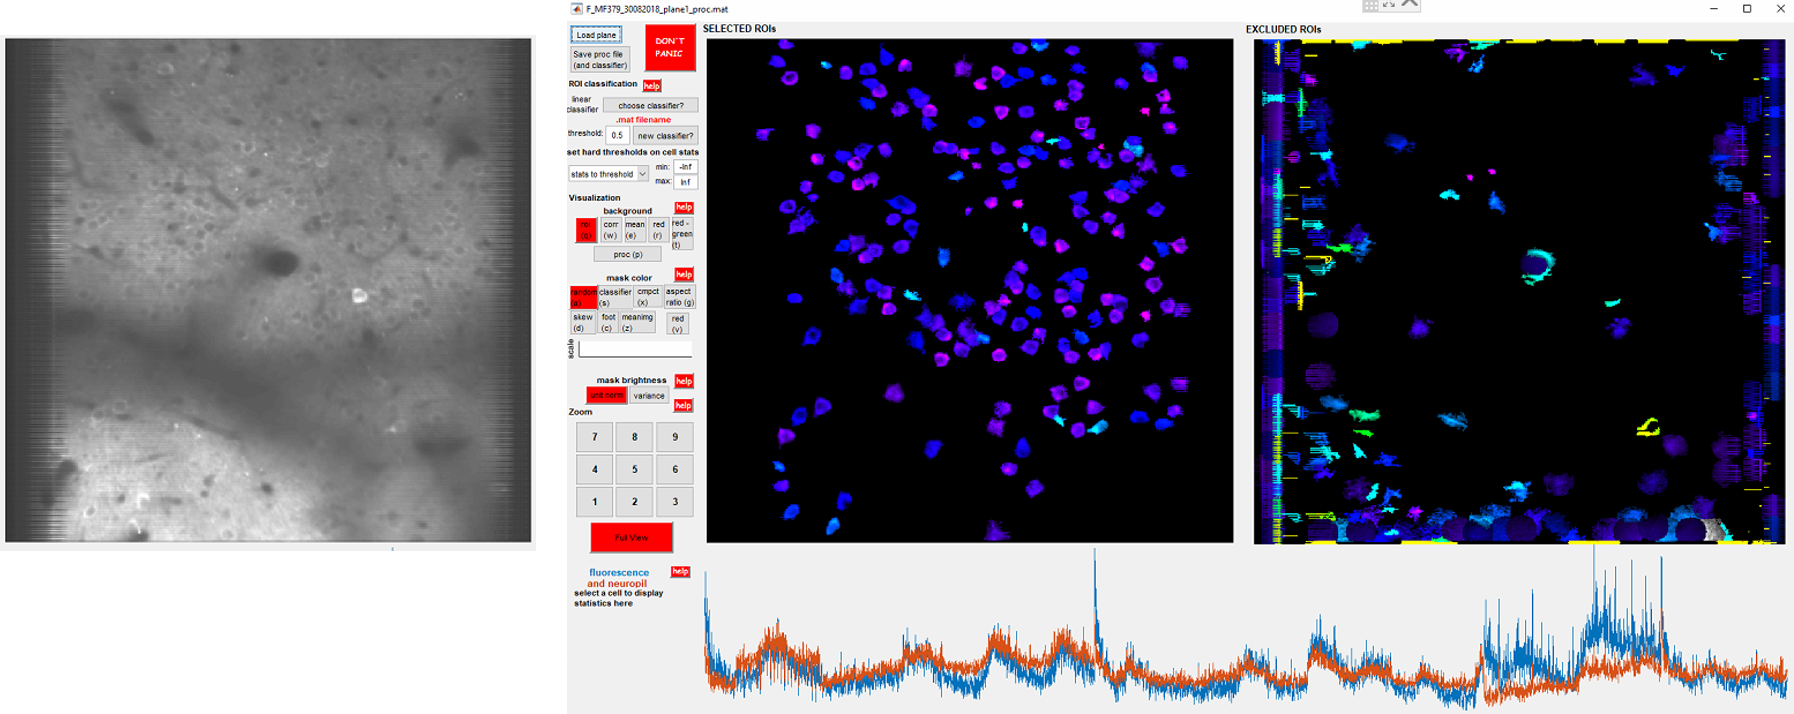
\includegraphics[width=13cm,height=13cm,keepaspectratio]{Figures/7.Results/ftraces/suit2p.png} 
%\caption{6_popPlots_Animal2_Session6} 
\end{figure}

Finally, the fourth stage of the pipeline outputs, for each ROI, a single calcium fluorescence time-varying signal. Again, this signal is corrected for the neuropil contamination signals. Furthermore, the spike train - the action potential sequence - that causes this signal is estimated, by use of a fitting model. 
A model is used for the uncorrected fluorescence $\vec{F}_i$, with a contribution by the convolution of the spike train $\vec{s}_i \geq 0$ with the calcium response kernel $\vec{k}_i$, a scalled neuropil and the noise:

\begin{equation}
    \vec{F}_i(t) = [\vec{s}_i * \vec{k}_i](t) + c_i \vec{N}_i (t) + noise
\end{equation}

To fit this model, $\vec{F}_i$ is extracted for each ROI i, the neuropil trace $\vec{N}_i$ is computed by averaging pixels in a ring shaped region around the ROI, and finally the coefficient $c_i$ and the spike train $\vec{s}_i$ are estimated for each cell by optimization of the cost function:

\begin{equation}
    Cost(\vec{s}_i, c_i)=||\vec{F}_i - \vec{s}_i * \vec{k}_i - c_i \cdot \vec{N}_i|| ^2 + \lambda \cdot L(\vec{s}_i)
\end{equation}

with $L(\vec{s}_i)$ a continuous, non-negative possible penalty on the spike train for each ROI.

In this way, the \textit{Suit2p} treatment of the raw movies produces a neuropil-corrected calcium trace $\vec{F}_i - c_i \vec{N}_i$, as well as the spike times estimates $\vec{s}_i$.

This processed data of fluorescence traces will be the substance for the posterior analysis.
\section{Data treatment}
\label{sec:DataTreatment}

Having the extracted neuropil corrected fluorescence traces, F, for all of the session's time, it is also required to extract $\Delta F/F$ traces: these indicate the measured changes in fluorescence between the cell's peak stimulation times and resting state and serve as the actual data measurements to use in all of subsequent analysis.

For every ROI's trace response, the baseline fluorescence ($F_0$) was estimated by discarding the tails of the fluorescence trace distribution and taking the mean fluorescence, using a 60 s sliding window. The obtained value was then used to calculate $\Delta F/F$ traces ($\dfrac{F-F_0}{F_0}$) for each cell (figure \ref{dfoverf}, left).

Cell  $\Delta F/F$ responses are thus mostly distributed around zero, with positive tails corresponding to spike responses (for an example cell $\Delta F/F$ distribution, figure \ref{dfoverf}, right).


\begin{figure}[H] \centering 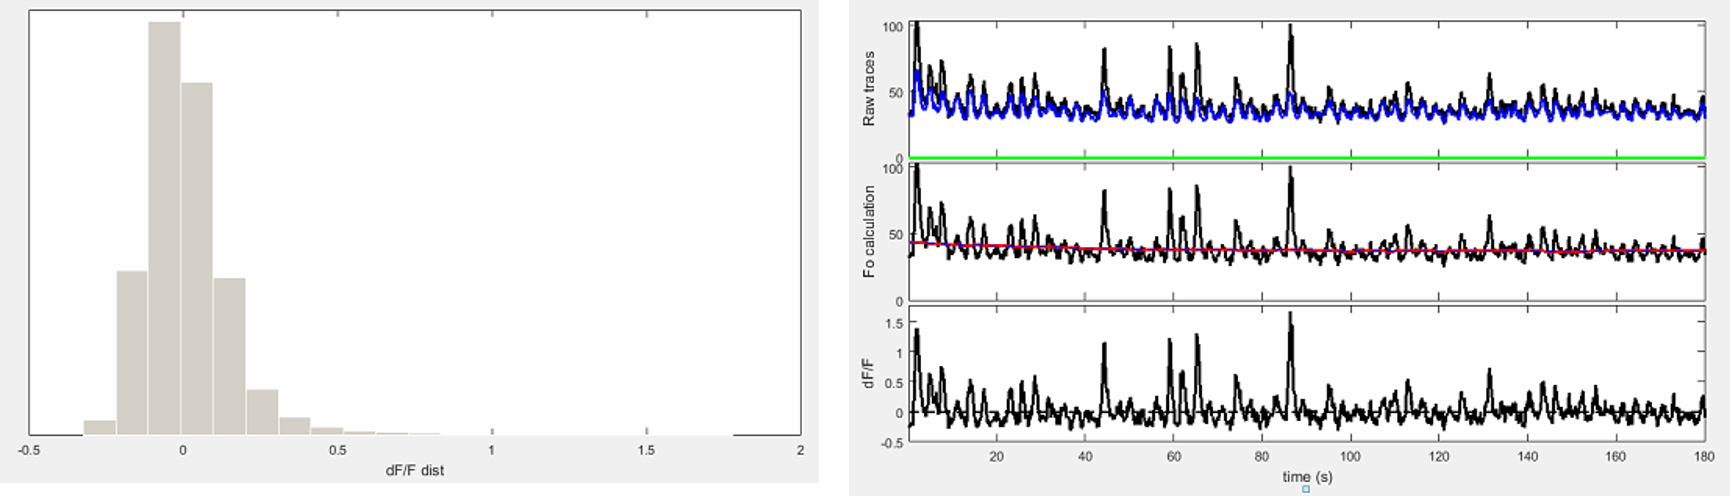
\includegraphics[width=15cm,height=15cm,keepaspectratio]{Figures/7.Results/ftraces/dFoverF.png} 
\caption{$\Delta F/F$ computation and results for an example ROI.
\newline \textbf{Left:} \textbf{Top} First 3 minutes section of raw fluorescence trace, F, for the example ROI (black trace) superimposed with the fluorescence baseline estimation trace for that ROI done by using a 60 s sliding window to discard trace's tails (blue trace); \textbf{Middle} Same fluorescence trace (black trace) superimposed with the baseline estimation value, $F_0$ (red trace), calculated as the average result of the baseline estimation trace in the top panel's blue trace, over the full session; \textbf{Bottom} $\Delta F/F$, computed as $\dfrac{F-F_0}{F_0}$.
\newline \textbf{Right:} Example ROI's $\Delta F/F$ distribution histogram. Cell's responses are mostly distributed around zero, with positive tails corresponding to spike responses.
\label{dfoverf}}
\end{figure}

Reviewing the process, we start with intrisic optical imaging on the subjects, to assess each animal's retinotopy maps and find the corresponding center field of view V1 encoding locations. 

We use two-photon imaging at that found location (with more thorough search for the center locations with the tuning protocol), and acquire brain recording sets of images of that brain's location GCaMP6s activity-related fluorescence values, for 4 different depth planes, while the subjects are shown stimuli (RF, tuning and SM protocols). 

These extracted raw images are then registered, and run through Suit2p pipeline, to select ROIs according to pixels temporal and spacial correlations in the image. These ROIs' pixels' fluorescence levels are averaged over that region and neuropil corrected. This results in raw fluorescence traces over the session's time.

With these, $\Delta F/F$ responses are computed. These are the processed data to map to the presented stimuli and use in the following analysis.

\section{RF analysis}

At each session's end, a RF analysis was held to assess whether the V1 imaged position corresponded to neurons with RFs centred in the center of the visual field, as these were the fixed intended positions for the subsequent SM spatial structure analysis.

Responses of each ROI were baseline subtracted and analysed trial by trial, mapping each trial's response to the visual field position that the corresponding stimulus was presented at (figure \ref{rfanalysis}, left panels).

Then, these responses were averaged over repetition trials, portraying mean response levels for each of the visual field positions (figure \ref{rfanalysis}, middle panels).

Finally, normalized gray-scale maps were produced for the response maps $R(az, el)$, with $az$ and $el$ the azimuth and elevation retinotopic coordinates, averaging over time on each of the positions' mean trace responses (figure \ref{rfanalysis}, right panels).

\begin{figure}[H] \centering 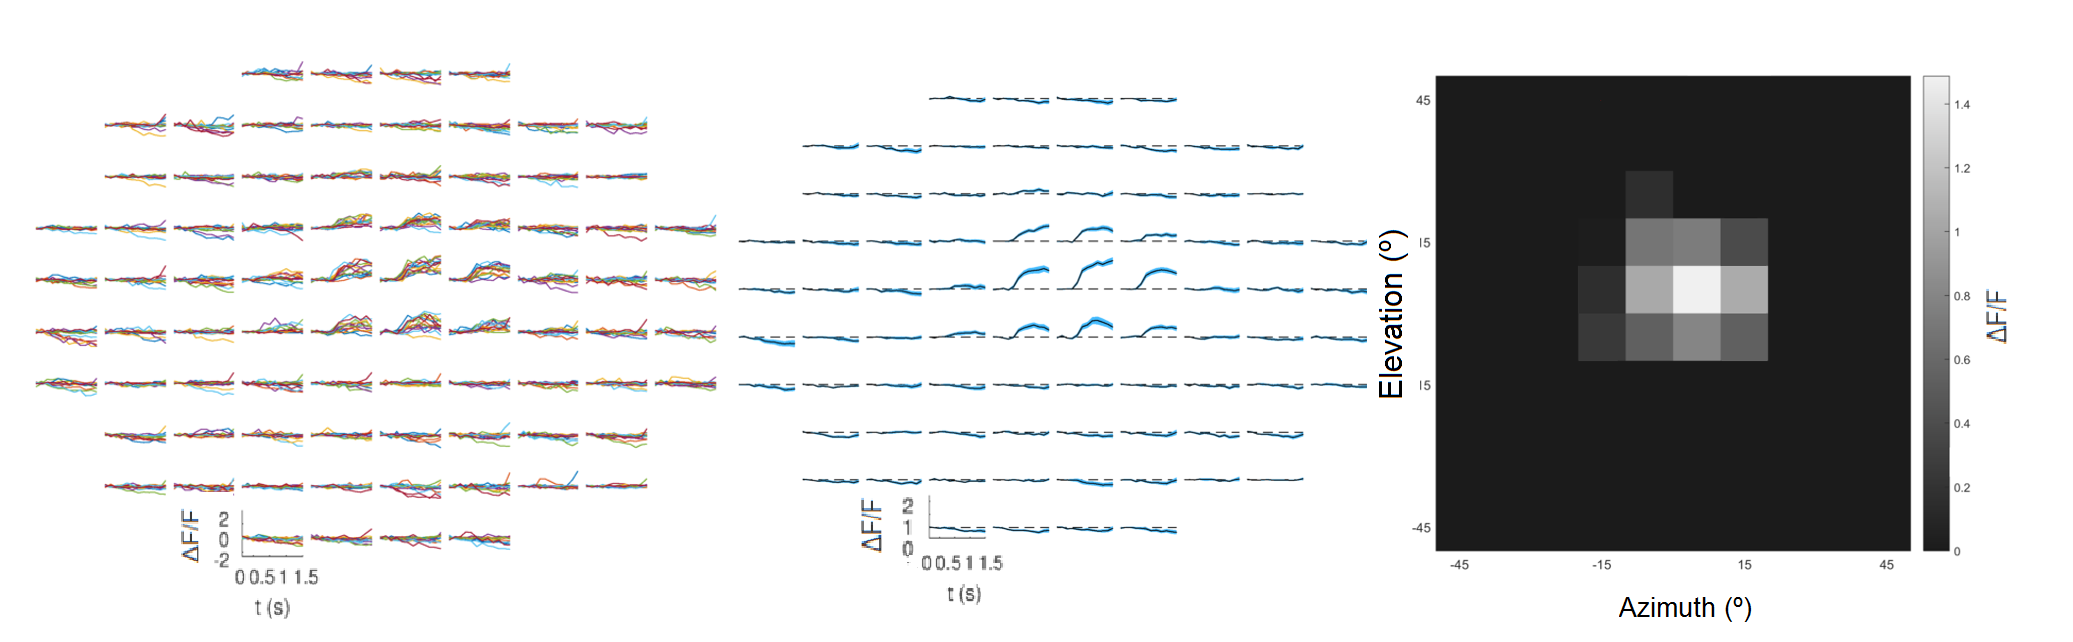
\includegraphics[width=16.2cm,height=16.2cm,keepaspectratio]{Figures/7.Results/rf/rf1.png} 
\caption{Example cell with well centred RF. 
\newline \textbf{Left:} Individual traces. Each of the 14 trial-type repetition trace response is represented in a different colour, for each of the visual field stimulated region. 
\newline \textbf{Middle:} Mean traces. Average traces over the 14 repetitions, represented also for each azimuth and elevation center stimulus condition. 
\newline \textbf{Right:}RF map. Response strengths to each of the stimulus positions, in a gray-scaled colour map.}
\label{rfanalysis}
\end{figure}

Each of these neurons' response maps was fitted to 2D-Gaussian ellipses, using Matlab implementation of the least-squares Levenberg-Marquardt algorithm (as in \cite{Marques2018}):

\begin{dmath}
R(az,el)=a+b\times \exp \left[ - \left( \dfrac{az-az_0}\times \cos(\theta)+ el-el_0)\times \sin(\theta){\sqrt{2} \times \sigma_1}\right)^2 - \left( \dfrac{-(az-az_0) \times sin \theta + (el-el_0)\times \cos(\theta)}{\sqrt{2} \times \sigma_2}\right)^2\right]
\end{dmath}

with $(az_0, el_0)$ the 2D Gaussian center coordinates, $\sigma_1$ and $\sigma_2$ the standard deviations of the gaussian across the two dimensions, $\theta$ the rotation angle between the gaussian and the $(az,el)$ axis, $a$ an offset parameter and $b$ an amplitude parameter.

The RF was then defined as the ellipse centred at $(az_0, ele_0)$ and limited by the standard deviations  ($\sigma_1$, $\sigma_2$):

\begin{equation}
\left[ \left( \dfrac{(az-az_0)\cdot \cos(\theta) + (el-el_0)\cdot \sin(\theta)}{\sigma_1}\right)^2 + \left(\dfrac{-(az-az_0)\cdot \sin(\theta) + (el-el_0)\cdot \cos(\theta)}{\sigma_2}\right)^2\right]=1
\end{equation}

The subsequent analysis was restricted to fits with $R^2>0.5$, as lower values corresponded to RF unreliable estimations. Within 10 sessions with 4 planes each, across 4 animals, 3168 out of 4198 dataset ROIs ($75\%$) were considered.

Analysing plane by plane, for each animal and session (example planes in figure \ref{ellipses}), one could assess that most of the considered RF centres were placed with similar centres within the retinotopical space, as theoretically expected for the short distances of $200 \times 200) \mu m$ imaged V1 planes. 

Two of the sessions showed very high elevation RFs, and were thus discarded for subsequent analysis, leaving 2772 measured RF cells and a total of 3728 cells ($74\%$ fitted RFs) to be analysed in regards to SM effects.

\begin{figure}[H] \centering 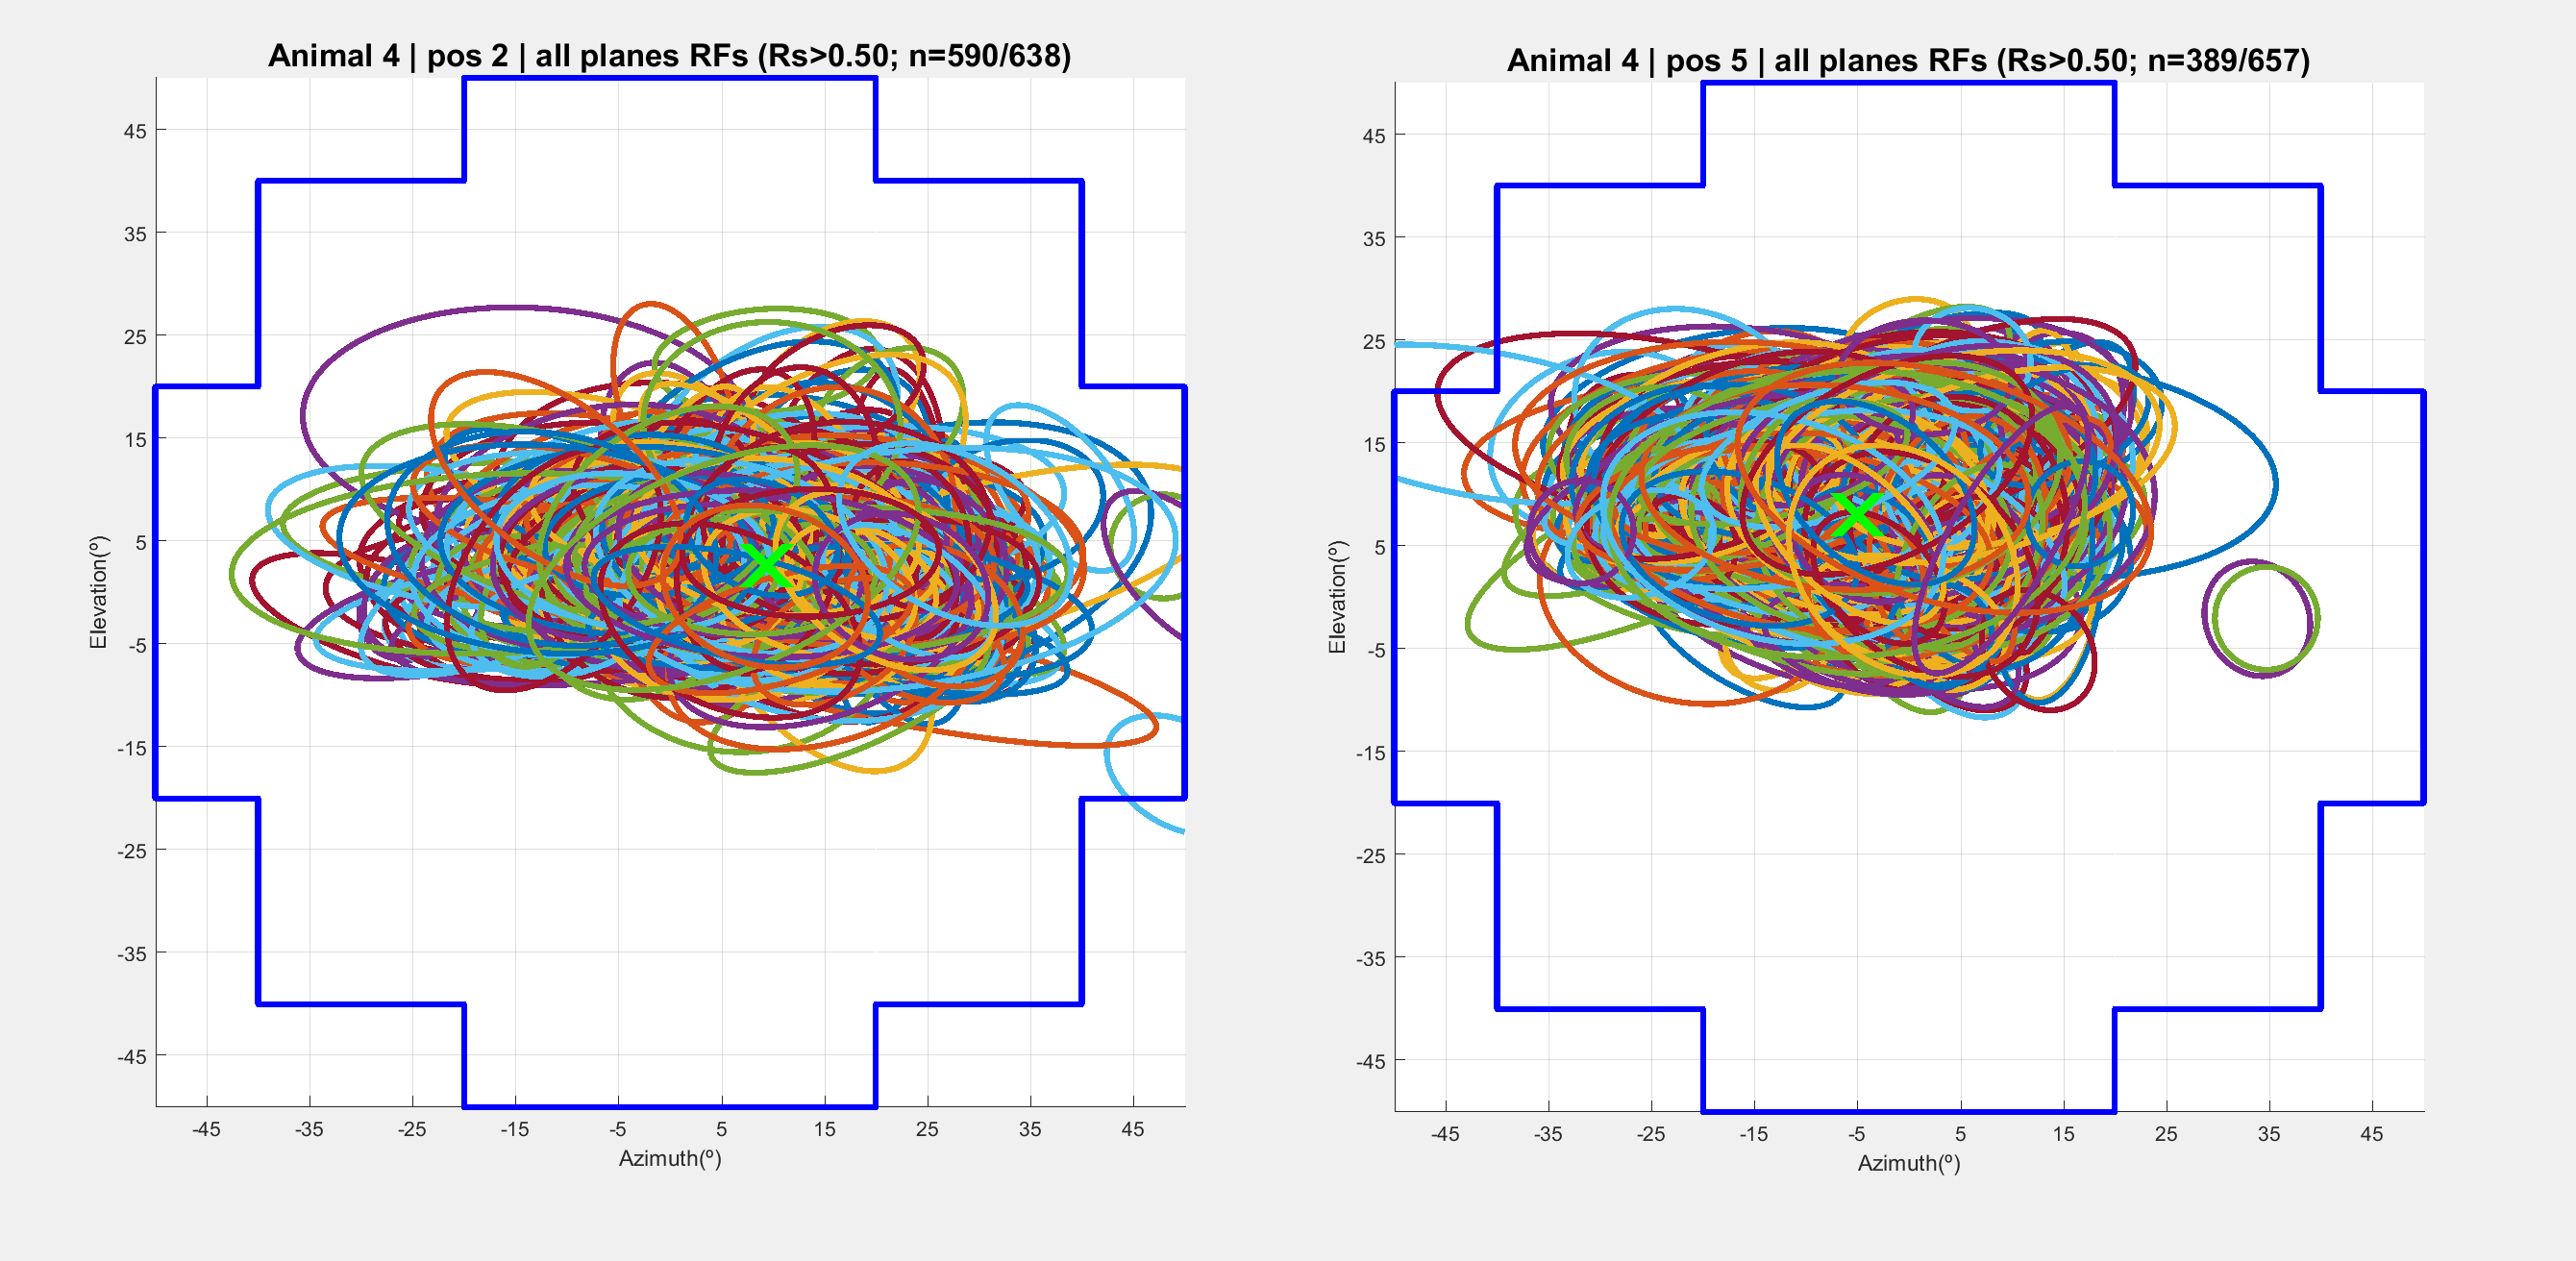
\includegraphics[width=13cm,height=13cm,keepaspectratio]{Figures/7.Results/rf/ellipsesAnimal4pos2andpos5.png} 
\caption{Superimposed 2D gaussian ellipsoidal fits for each neuron in the same plane. Two planes from two different sessions with the same animal are presented as examples.}
\label{ellipses}
\end{figure}

\section{Tuning analysis}
\label{tuningresults}

To validate bpod's tuning protocol, the selected neurons were analysed in regards to their direction (8 directions), spatial (2) and temporal (2) frequencies tuning selectivity.

Neurons in V1 can have orientation selectivity (\cite{Hubel1959}, \cite{Hubel1962}), that is, respond more strongly to a preferred orientation than to any other orientation. For mice, these orientation-selective (OS) cells are not organized into functional columns as they are for carnivores and primates (\cite{Hubel1962}), yet they do present strong orientation selectivity.

Moreover, a subset of  OS cells are also direction-selective (DS): these respond most strongly to a preferred direction than to any other.

For orientation analysis, responses of opposite directions are averaged together, and ploted on polar coordinates (figures \ref{tuninganalysisOS} and \ref{tuninganalysisDS}). The vector sum of responses at each individual trial (combining the trials for each of the same orientation opposed directions) then forms the \textit{orientation vector} of that trial. The orientation vectors for all trials then exhibit the cell's orientation tuning properties.
In the analogous way, for direction analysis, each trial measurement is binned to different direction labels, and the vector sum of the responses at individual directions then amounts to a direction vector for each trial. Direction vectors for all trials represent the cell's direction tuning properties.

Statistical significance is assessed with vector-based Hotelling's $t^2$-tests with confidence of 95\% in this project's case, to ask whether the 2D mean of the distribution of orientation and or direction vectors differ from (0,0).
 
 For any orientation, if the responses to a given orientation are significantly higher than responses to any other orientation, then the former is called the neuron's preferred orientation. This differential effect can be measured with an orientation selectivity index (OSI), for the preferred orientation response in the considered space. With  $R_{pref_or}$ the responses to the preferred orientation and $R_{orth}$ the responses to the orientation orthogonal to the preferred:
\begin{equation}
\text{OSI}= \dfrac{R_{pref \_or} - R_{orth}}{R_{pref \_or} + R_{orth}}
\end{equation}

Similarly, in the direction space, a preferred direction can also be determined for neurons that have significantly higher responses in one direction than they do in the null direction relative to the former. A DSI can be computed, for the direction doublet:

\begin{equation}
\text{DSI}=\dfrac{R_{pref} - R_{null}}{R_{pref} + R_{null}}
\end{equation}

In regards to the spatial and frequency tuning, here we used a restricted $(2 \times 2)$ space and found that for most cells, in this space, the preferred spatial frequency was of 0.04 cycles per degree and the preferred temporal frequency was at 1 Hz. These were the frequency specifications used in both the RF protocol and the SM protocol.

Here, we present two example cell responses for the different stimulus conditions in the tuning protocol: an OS cell (figure \ref{tuninganalysisOS}) and a DS cell (figure \ref{tuninganalysisDS}).

\begin{figure}[H] \centering 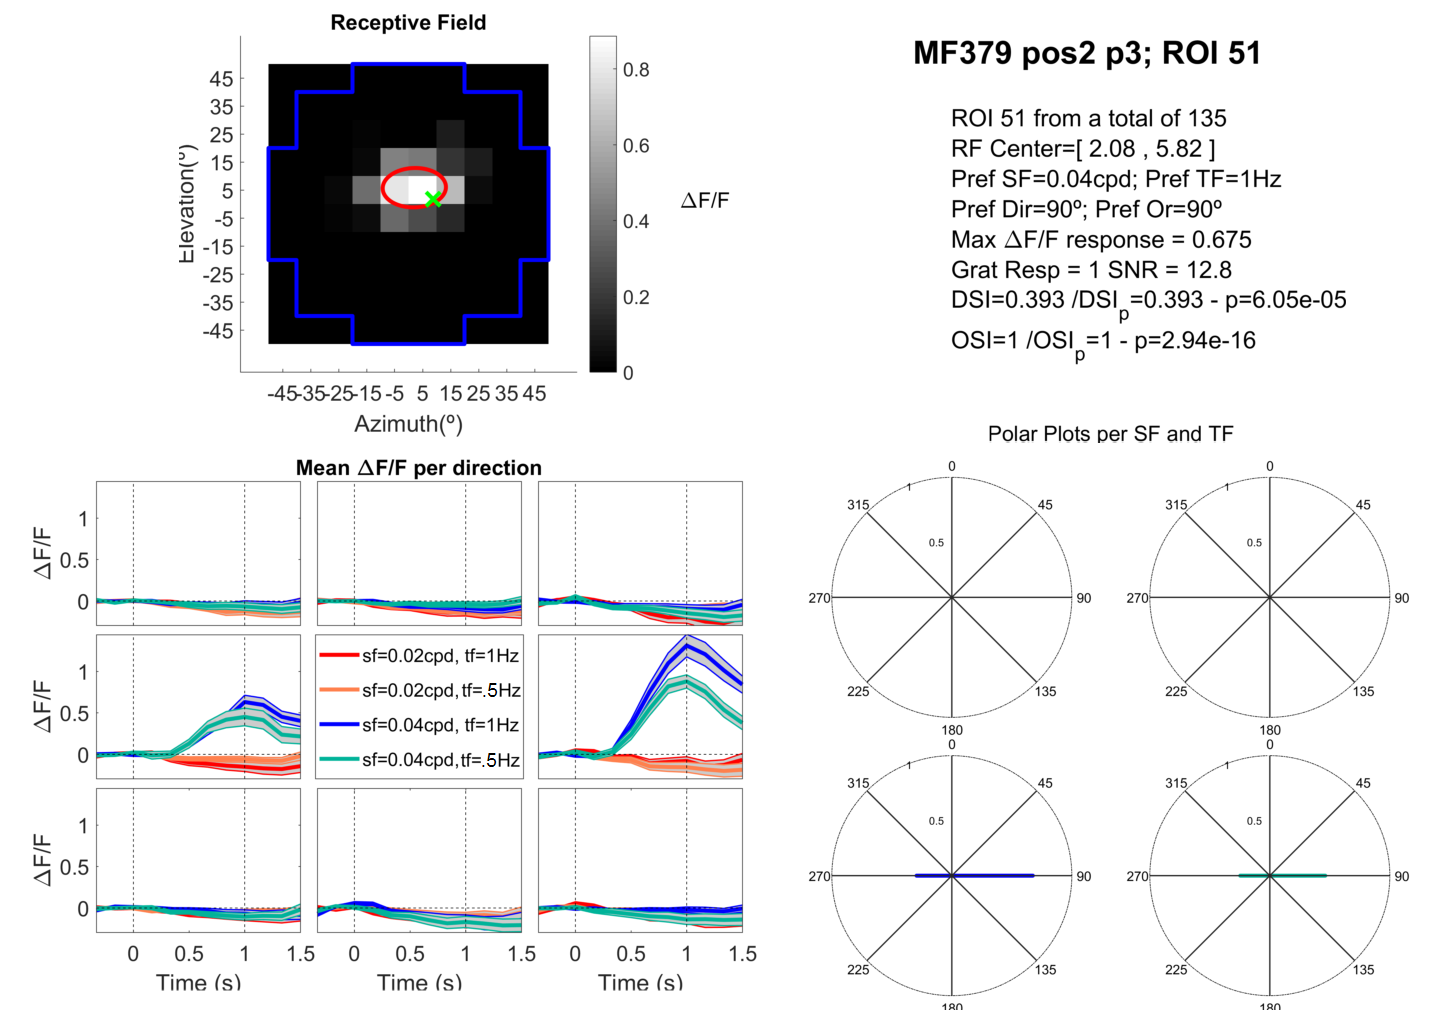
\includegraphics[width=12cm,height=12cm,keepaspectratio]{Figures/7.Results/tuning/MF379_pos2_p3_ROI0051.png} 
\caption{Tuning analysis for an example OS cell. Preferred $SF=0.04 cpd$, $TF=1 Hz$, up direction and vertical orientation. $DSI=1$ ($p=1.87 \cdot 10^{-5}$), $OSI=0.967$ ($p=3.4 \cdot 10^{-4}$).}
\label{tuninganalysisOS}
\end{figure}

\begin{figure}[H] \centering 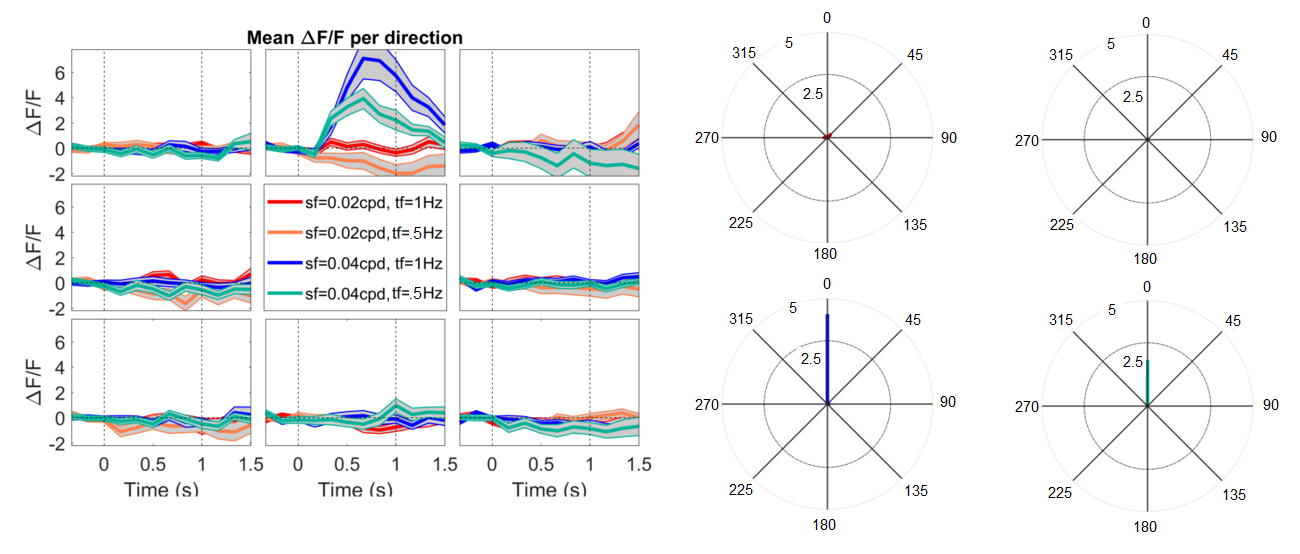
\includegraphics[width=12.5cm,height=12.5cm,keepaspectratio]{Figures/7.Results/tuning/CM006_pos1_p4_ROI0138.png} 
\caption{Tuning analysis for an example DS cell. Preferred $SF=0.04 cpd$, $TF=1 Hz$, temporal direction and horizontal orientation. DSI=0.393 ($p=6.05 \cdot 10^{-5}$), OSI=1 ($p=6.05 \cdot 10^{-5}$).}
\label{tuninganalysisDS}
\end{figure}

\subsection{Surround modulation analysis}
\label{cap:Methods}

SM analysis started with the mapping of responses during the protocol to corresponding stimuli types, from the 124 possible ones. During the experiments, 20 repetitions were held for most sessions. However, in the analysis, it was noticeable that responses decreased a lot in the second part of the protocol, possibly due to anaesthesia cumulative effects and/or adaptation to the stimuli. Therefore, to prevent from adding noise to averaged measurements, the subsequent analysis was using only the 10 first repetitions of each trial type.

Trial types were ordered in a given structure:

\begin{itemize}
\item \textbf{[1:4]} S1T, at the four directions (up, temporal, down, nasal); 
\item \textbf{[5:8]} C, analogous to above; 
\item \textbf{[9:12]} S1B, analogous to above;
\item \textbf{[13:16]} S1L, analogous to above;
\item \textbf{[17:20]} S1R, analogous to above; 
21:36 S1T+C, with first quarter (21:24) center up and surround in the 4 directions (up, temporal, down, nasal), second quarter (25:28) center temporal and surround in the 4 directions, third quarter (29:32) center down and surround in the 4 directions, and fourth quarter (33:36) center nasal and surround in the 4 directions;
\item \textbf{[37:52]} S1B+C, analogous to above;
\item \textbf{[53:68]} S1L+C, analogous to above;
\item \textbf{[69:84]} S1R+C, analogous to above;
\item \textbf{[85:100]} S2H+C, with first quarter (85:100) center up and the two horizontally positioned surrounds in the same of 4 directions (up, temporal, down, nasal), second quarter (89:92) center temporal and surrounds in the same of 4 directions, third quarter (93:96) center down and surrounds in the same of 4 directions, and fourth quarter (97:100) center nasal and surrounds in the the same of 4 directions;
\item \textbf{[101:104]} S2H, at the four directions (up, temporal, down, nasal);
\item \textbf{[105:120]} S2V+C, with first quarter (105:108) center up and the two vertically positioned surrounds in the same of 4 directions (up, temporal, down, nasal), second quarter (109:112) center temporal and surrounds in the same of 4 directions, third quarter (113:116) center down and surrounds in the same of 4 directions, and fourth quarter (117:120) center nasal and surrounds in the the same of 4 directions;
\item \textbf{[121:124]} S2V, at the four directions (up, temporal, down, nasal);
\end{itemize}
\chapter{Statistical Tests}
\label{chapter:StatisticalTests}

Along the SM analysis, statistical tests were used to test given hypothesis, assess results significance and perform multiple comparisons. These tools were implemented with Matlab ingrained functions (\texttt{signtest}, \texttt{ranksum}, \texttt{anovan}, \texttt{corrcoef} and \texttt{regress}). Here we summarily review these tools and underlying mathematical basis.

\section{Two-sided sign-tests}
\label{subsec:signtests}

Sign-tests are nonparametric tests, for given independent observations, for the hypothesis that the difference between the correspondent variables has a given median value $\eta_0$. In this work's analysis, the hypothesized median was zero. 

In this test, the only assumption is that data is collected independently from a continuous distribution.

For a two-sided test, as used in this project's analysis, the null hypothesis and alternative hypothesis are given by:

H_0 : $\eta = \eta _0$

H_a : $\eta \neq \eta _0$

We define $S_1$ the counts of the number of observations less than $\eta _0$ and  $S_2$ the counts of the number of observations larger than $\eta _0$. 

The test statistic is the given by:

\begin{equation}
S=max(S_1, S_2)
\end{equation}

If the null hypothesis $H_0$ is true, then S follows a binomial distribution $S ~ \text{Binomial} (m, 0.5)$, with $m$ the number of observations, discarding the data points equal to $\eta _0$.

Then, in general, the p-value, \textit{p}, is defined by

\begin{equation}
p=2 \text{Pr}\left[ X \geq S \right]
\end{equation}

and we reject the null hypothesis $H_0$ if \textit{p} is smaller or equal to a given significance threshold $\alpha$.

For large samples, as is the case for this project's data sets, it can be shown that if X ~ Binomial (m, 0.5), then the distribution can be approximated by X ~ Normal (0.5m, 0.5(1-0.5)).

Then, the continuity corrected (replacing $S$ by $S-0.5$) z-statistic can be used:

\begin{equation}
Z=\dfrac{S-E(S)}{\sqrt{V(S)}}= \dfrac{(S-0.5m - 0.5 sign(n_+-n_-))}{\sqrt{(0.5)(0.5)m}}
\end{equation}

with $E(S)$ and $V(S)$ respectively the expected value and the variance, ($V(S)=E(S^2)-(E(S))^2$)of the random variable S, m the number of elements, $n_{+}$ and $n_{-}$ respectively the number of positive and negative differences from the hypothesized median value.

This statistic follows a normal distribution Z~Norm(0, 1), if the null hypothesis is true. 

The p-value can thus be defined, for large data sets:

\begin{equation}
p = 2 \text{Pr}\left[X \geq Z\right]
\end{equation}

and we again reject the null hypothesis $H_0$ if \textit{p} is smaller or equal to a considered significance threshold $\alpha$.

\section{Wilcoxon signed rank-sum tests}
\label{subsec:subbsectionC}

Wilcoxon signed rank-sum tests are non-parametric tests used when collected data samples $(y_{11},...,y_{n1})$ and $(y_{12},...,y_{n2})$ is expected to be dependent, that is, data is \textit{paired}.

As for the last test, the only assumption here is that data is collected independently from a continuous distribution.

Fist, for the n sized data set, we compute the within-individual differences, for $i=1,...,n$, $x_i = y_{i1} - y_{i2}$ and discard any data point for which $x_i=0$, adjusting the sample size - let's call it $m$.

Then, the absolute values of $x_1,...,x_m$ are sorted into ascending order, and labelled with a rank from 1 to $m$. In the case of ties, average ranks are given.

Next, we define two rank sums:

$T_+ =$ Sum of ranks for which $x_i>0$

$T_-$ = Sum of ranks for which $x_i<0$

The null hypothesis is then posed:

\begin{center}
$H_0$: No change between the two measurements
\end{center} 

and put against three alternative hypothesis: $H_a(1)$ significant decrease, $H_a(2)$ significant increase and $H_a(3)$ significant change between the two measurements.

Critical $T_0$ values are tabled. If $T_- \leq T_0$, we reject $H_0$ in favour of $H_a(1)$; if $T_+ \leq T_0$, we reject $H_0$ in favour of $H_a(2)$; and finally, with a two-sided test with $T=min(T_-, T_+)$, if  $T \leq T_0$, we reject $H_0$ in favour of $H_a(3)$.

For large sample tests, as is the case, the algorithm uses a Z statistic:

\begin{equation}
Z = \dfrac{T_+ - \dfrac{m(m+1)}{4}}{\sqrt{\dfrac{n(m+1)(2m+1)}{24}}}
\end{equation}

If $H_0$ is true, Z can be approximated by a normal distribution Z ~ Normal(0,1), with different tabled critical values for each of the alternative hypothesis tested with.

In Matlab's algorithm, continuity correction and tie adjustments are also used, and the tests are carried in an analogous way.

\section{N-way analysis of variance}
\label{subsec:subcsectionC}

An n-way analysis of variance (ANOVA) is an extension on the one-way ANOVA. This conservative statistical tool examines the effect of n categorical independent variables on one continuous dependent variable. This results in not only an estimation of each categorical variable's influence but also assesses the influence of the interactions between these variables.

A n-way ANOVA determines if a data set differs as a function of groups of n factors. A n-way ANOVA can be generalized from a two-way ANOVA. For 3 factors A, B and C, for example, a model can be written as:

\begin{equation}
y_{ijkr}=\mu + \alpha_i + \beta_j + \gamma_k +(\alpha \beta)_{ij}+(\beta \gamma)_{jk}+(\alpha \beta \gamma)_{ijk}+\epsilon_{ijkr}
\end{equation}

with $y_{ijkr}$, an observation of the response variable; $i$, $j$ and $k$ representing respectively groups from factors A, B and C and r the replication number; $\mu$ the overall mean; $\alpha_i$, $\beta_j$ and $\gamma_k$ respectively the deviations of groups of factor A, B or C from $\mu$ due to corresponding factors A, B or C. $\epsilon_{ijkr}$ are the random disturbances, assumed independent, normally distributed and with constant variance. The 2-way and 3-way interactions between factors are accounted for in the model, within the other terms of the model equation, respectively with two subscripts and three subscripts.

A n-way ANOVA the tests 7 null versus alternative hypothesis:

The hypothesis about the equality of the mean response for groups of factor A, with I the number of groups in A:

\begin{center}
$H_0=: \alpha_1=\alpha_2...=\alpha_I$

$H_a:$ at least one $\alpha_i$ is different, $i=1,...,I$
\end{center}

and the equivalent analogous for factors B and C.

The two-factors interaction hypothesis:

\begin{center}

$H_0$:$(\alpha \beta)_{ij}=0$

$H_a$: at least one$(\alpha \beta)_{ij}\neq 0$

\end{center}

and the equivalent analogous for other two-factor interactions.

Finally, the three-factor interaction hypothesis:

\begin{center}
$H_0$:$(\alpha \beta \gamma)_{ijk}=0$

$H_a$: at least one$(\alpha \beta \gamma)_{ijk}\neq 0$
\end{center}

\section{Pearson correlation coefficients}
\label{subsec:subcsectionC}

Correlation coefficients between two random variables A and B measure their linear dependence. For N scalar observations from each variable, the Pearson correlation coefficient is given by:

\begin{equation}
\rho(A, B) = \dfrac{1}{N-1} \sum_{i=1}^N \left( \dfrac{A_i - \mu _A}{\sigma _A}\right) \left( \dfrac{B_i - \mu_B}{\sigma _B}\right)
\end{equation}

with $\mu_A$ and $\sigma_A$ the mean and standard deviation of A, and $\mu_A$ and $\sigma_A$ the mean and standard deviation of B.

In matlab's algorithm, matrices of correlation coefficients are computed and the matrix of p-values for testing the null hypothesis that there is no relationship between the observed phenomena. If these p-values are smaller than the considered $\alpha$ threshold, the correlations are deemed significant.

\section{Multiple linear regression}
\label{subsec:subcsectionC}

Linear regression models describe the relationship between a dependent variable $y$, and $K$ independent variable(s) $X$.

A multiple linear regression model is given, for $i=1,...,n$, with n the number of responses, by:

\begin{equation}
y_i=\beta_0 + \beta_1 X_{i1}+...+\beta_p X_{ip}+\epsilon_i
\end{equation}

with $y_i$ the $ith$ response, $\beta_k$ the $k$th coefficient, $X_{ij}$ the \textit{i}th observation on the \textit{j}th independent variable, with $j=1,...,k$, and $\epsilon_i$ the random error term, assumed uncorrelated, independent and identically normal distributed. 

It follows that the fitted linear function is given, for $i=1, ..., n$ by:

\begin{equation}
\hat{y_i}= \sum _{k=0}^K b_k f_k(X_{i1},...X{ip})
\end{equation}

with $f$ a scalar-valued function of the independent variables, and K the number of independent variables.
\section{Permutation test}

When interested on strong null hypothesis, permutation tests can be conducted for assessing sampling distributions. This test builds sampling distributions by resampling the observed data. This is done with no replacement, by simply eliminating the outcome labels on the original sample data and then randomly redistributing the observed values under those same labels. This shuffling process can be repeated to obtain a large number of resamples.
Significance tests can then be used for the null hypothesis that these resample distributions do not differ from the original distribution.

\section{Multivariate comparisons: Holm-Bonferroni method}

Finally, in this work, many comparisons were held on different pools of the dataset. For this reason, the multiple comparisons problem needs to be accounted for: The more statistical inferences that are made simultaneously, the more likely it is for Type I error (false positive) inferences to be made. This issue steams from considering an overall confidence level for the whole set of simultaneous tests, while these threshold levels are to be considered individually. The controlled variable should be the familywise error rate (FWER), the probability of making one or more type-I errors, with a given significance level threshold, $FWER \leq \alpha$.

To compensate for this problem in the multivariate comparisons held, the Holm-Bonferroni method was used to adjust the rejection thresholds for each individual tested hypotheses. 

With $H_1,...,H_m$ a family of $m$ null hypothesis, and $p_1,...,p_m$ the corresponding p-values, we order the p values from lowest to highest $p_{(1)},...,p_{(m)}$, associated to the respective null hypothesis, $H_{(1)},...,H_{(m)}$.

For an established $\alpha$ significance level threshold, we let $k$ be the minimal index such that $P_{(k)}> \dfrac{\alpha}{m+1-k}$. Then, we reject the null hypothesis $H_{(1)}...H_{(k-1)}$. If $k=1$, no null hypothesis is rejected, and if no such $k$ exists, all null hypothesis are rejected. This method ensures that $FWER \leq \alpha$ has intended to appropriately assess the joint multiple inferences.
\cleardoublepage